\section{Background and Preliminaries}\label{sec:background}

Building carbon-aware LLM serving schedulers requires joining four domains that developed under separate abstractions: phase-level transformer execution, wide-area carbon routing, GPU serverless cold-start management, and lifecycle carbon accounting under ISO/IEC 21031:2024. Fig.~\ref{fig:architecture} illustrates how these layers interact inside the dual-track control architecture.

\begin{figure*}[t]
    \centering
    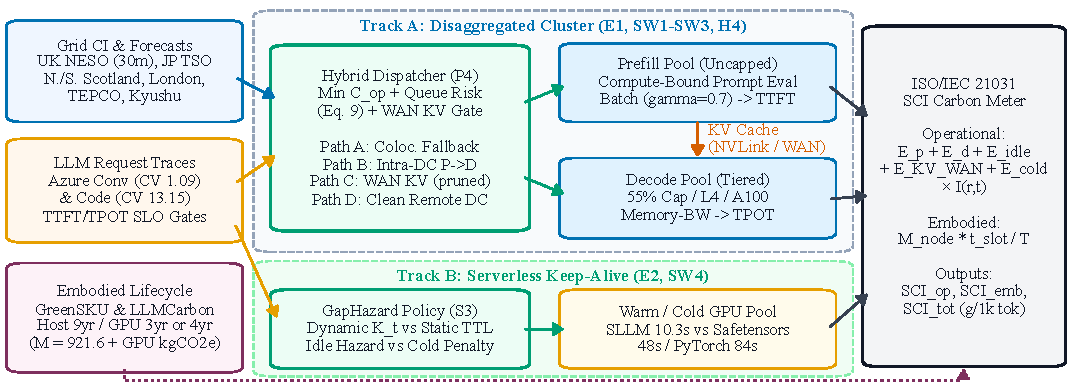
\includegraphics[width=\textwidth]{figures/fig1_architecture.pdf}
    \caption{Dual-track carbon-aware phase-disaggregated LLM cluster (Track A: Paths A--D via Eq.~\eqref{eq:dispatch}) and serverless GPU keep-alive (Track B: GapHazard policy \texttt{S3}) feeding the unified ISO/IEC 21031:2024 SCI telemetry meter.}
    \label{fig:architecture}
\end{figure*}

\subsection{Autoregressive LLM Phases and Disaggregation}\label{subsec:bg_phases}
Within multi-tenant cloud platforms~\cite{mell2011nist}, autoregressive LLM serving proceeds in two stages for each request with prompt length $L_{\text{in}}$ and generation length $L_{\text{out}}$. During \emph{prefill}, the model processes all $L_{\text{in}}$ prompt tokens concurrently through matrix multiplications to produce the first token and populate the KV cache, which determines time-to-first-token (TTFT). During \emph{decode}, the engine iterates token by token over $L_{\text{out}}$ steps, reloading model weights and the growing KV cache from high-bandwidth memory (HBM) on each step; this saturates memory bandwidth before arithmetic units and governs time-per-output-token (TPOT).

Production traces show strong workload skew across domains: Azure LLM logs report conversational prompts averaging $1{,}154.7$ input and $211.1$ output tokens with steady arrivals (coefficient of variation $\text{CV}=1.094$), whereas coding completions average $2{,}047.8$ input and $27.9$ output tokens under extreme burstiness ($\text{CV}=13.152$)~\cite{azure2024trace}. Mooncake traces exhibit even heavier prompt skew, averaging $8{,}590$ input versus $182$ output tokens~\cite{qin2025mooncake}.

Local memory and batching schedulers address single-cluster bottlenecks first. PagedAttention in vLLM cuts KV waste from 61.8\%--79.6\% down to 3.7\% and saves up to 55.2\% KV memory via copy-on-write~\cite{kwon2023vllm}, while Sarathi-Serve uses chunked prefill and stall-free batching to eliminate 28.3$\times$ generation stalls~\cite{agrawal2024sarathi}. Even with chunked batching, colocated requests couple prefill latency spikes with decode tail violations and restrict hardware specialization.

Phase-disaggregated architectures (Splitwise~\cite{patel2024splitwise}, DistServe~\cite{zhong2024distserve}, Mooncake~\cite{qin2025mooncake}, and DualScale~\cite{basit2026dualscale}) separate prefill and decode onto distinct GPU pools connected via NVLink or RDMA fabrics. Splitwise shows that decode GPUs tolerate a 50\% power-cap drop (700~W down to 350~W on H100) with minimal TPOT impact while achieving 2.35$\times$ iso-power-cost throughput~\cite{patel2024splitwise}; DualScale cuts prefill energy by 39\% and decode energy by 48\% at P99 latency parity~\cite{basit2026dualscale}. Empirical measurements confirm that decode still dominates cumulative energy across token ratios~\cite{fernandez2025acl}, and bilinear $(L_{\text{in}}, L_{\text{out}}, L_{\text{in}}L_{\text{out}})$ energy regression achieves $R^2 \ge 0.964$~\cite{wilkins2024offline}. However, recent dual-GPU experiments by Li et al.~\cite{li2026revisiting} caution that disaggregation can underperform colocated inference at small batch sizes over constrained interconnects until batch-32 KV eviction pressure triggers colocation collapse.

\subsection{Wide-Area Carbon Routing and KV Transfer Economics}\label{subsec:bg_wan}
Regional electricity grids vary widely in hourly operational carbon intensity $I(r,t)$ ($\text{gCO}_2\text{eq/kWh}$). Across 123 Electricity Maps grids, Sukprasert et al.~\cite{sukprasert2024limitations} report a 40$\times$ spread (mean $368.39\text{ gCO}_2\text{eq/kWh}$) and note that 87\% of 40 sampled datacenter grids exhibit 24-hour periodicity. Yet latency and capacity constraints sharply curtail pure carbon-chasing: unconstrained 96\% spatial reductions shrink to 51.5\% under 50\% regional spare capacity and 31\% under a \SI{50}{\milli\second} WAN round-trip time (RTT) ceiling, while 50\% grid-forecast error introduces 10\%--12\% overhead~\cite{sukprasert2024limitations}.

Live multi-region Kubernetes scheduling in GreenCourier cuts carbon by 8.7\%--17.8\% across four European zones at a 10.3\%--16.2\% latency penalty~\cite{chadha2023greencourier}, whereas single-cluster temporal deferrals~\cite{wiesner2021letswait}, elastic scaling~\cite{hanafy2023carbonscaler}, battery orchestration~\cite{souza2023ecovisor}, and microservice DAG routing~\cite{gsteiger2024caribou} rely on delay tolerance or small HTTP payloads. In cloud-to-edge continuums, linear-programmed function variant selection lets 30\% more requests satisfy QoS targets and cuts execution carbon by 20\% under equal budgets~\cite{calavaro2026offloading}.

For LLM serving, splitting prefill and decode across WAN regions adds serial KV-cache transmission: a 70B-class FP16 GQA KV state at long context spans hundreds of megabytes per request, adding both WAN transmission latency ($L_{\text{kv}}/B_{\text{wan}}$) and network transfer energy (0.001--0.005~kWh/GB~\cite{gsteiger2024caribou}). Cross-region disaggregation is therefore beneficial only when the carbon savings between regions exceed network transfer emissions without breaching TTFT SLOs.

\subsection{Serverless GPU Keep-Alive and Checkpoint Loading}\label{subsec:bg_serverless}
Under bursty traffic, such as Azure Functions where 81\% of apps see $\le 1\text{ req/min}$~\cite{shahrad2020serverless}, idle servers draw static power while eviction incurs cold-start energy. In Kepler benchmarks, idle CPU draw reaches 21\%--83\% of peak power~\cite{sun2026lacere}, and an idle GPU draws 60--100~W. For 70B-class LLMs (about 130~GB weights), checkpoint cold-start duration spans 84.0~s under standard PyTorch loading, 48.0~s under Safetensors, and 10.3~s even with ServerlessLLM NVMe RAID-0 Direct I/O~\cite{fu2024serverlessllm}.

Recent dynamic keep-alive controllers (EcoLife~\cite{jiang2024ecolife}, CASA~\cite{qi2024casa}, LowCarb~\cite{roy2026lowcarb}, LACE-RL at -77.08\% idle carbon~\cite{sun2026lacere}, and Festina at -56\% energy and -85\% cold starts~\cite{wang2026festina}) show that adaptive idle timeouts outperform fixed windows, yet systematic comparison across multi-gigabyte loader tiers and clean versus coal-heavy grids remains open.

\subsection{ISO/IEC 21031:2024 SCI and Embodied Carbon}\label{subsec:bg_sci}
To prevent shifting emissions between operational and hardware budgets, the Green Software Foundation Software Carbon Intensity (SCI) specification, standardized as ISO/IEC 21031:2024~\cite{iso2024sci}, mandates an additive lifecycle intensity per functional unit $R$ (here, 1,000 processed tokens) while explicitly excluding offset purchases:
\begin{equation}\label{eq:sci}
\text{SCI} = \frac{(E \cdot I) + M}{R},
\end{equation}
where $E$ is total consumed electricity ($\text{kWh}$, inclusive of datacenter PUE), $I$ is regional grid carbon intensity ($\text{gCO}_2\text{eq/kWh}$), and $M = M_{\text{server}} \cdot (t_{\text{slot}}/T_{\text{life}})$ is amortized manufacturing carbon.

Industry GHG audits~\cite{gupta2021chasing}, architectural models~\cite{gupta2022act,acun2023carbonexplorer}, and LLM carbon tools~\cite{faiz2024llmcarbon,li2025ecoserve} show that embodied emissions (800~kgCO$_2$eq host baseline~\cite{li2025ecoserve}; 921.6~kgCO$_2$eq in the GreenSKU Genoa assembly, plus die/HBM~\cite{faiz2024llmcarbon}) represent 24\%--35\% of LLM totals on average grids and surpass 80\% as grids decarbonize. Consequently, metrics using raw GPU utilization~\cite{sinha2025utilization} or ignoring power capping~\cite{kakolyris2025throttllem,stojkovic2025dynamollm,stojkovic2025tapas} and aging amortization~\cite{hewage2025aging,li2023clover} risk optimizing local Watts while raising system-wide lifecycle carbon. These tradeoffs motivate unified simulation testbeds in the tradition of CloudSim~\cite{calheiros2011cloudsim}.
